\section*{Phase plane analysis}
\addcontentsline{toc}{section}{Phase plane analysis}

In order to get the phase plane of the network we determined the fixed points by setting $\frac{dS_{1}}{dt} = 0$ and $\frac{dS_{2}}{dt} = 0$. $Fig 3$ shows the development of the phase plane starting from no external input to stimulus with increasing coherence. \\

In the absence of external stimulus the network has \textbf{five fixed points} out of which 3 are attractors and 2 are repellers. $Fig 2.A$ shows the phase plane when no external stimulus is present.At this stage the network is unbiased and lies on the lower left attractor point (spontaneous stage). The other two attractors corresponds to those points where one of the neuron population shows self sustained behaviour.\\

$Fig 2.B$ shows the phase plane when it has an unbiased external stimulus. Under such condition, the spontaneous stable point and the repellers collapses to form a saddle point. The two diagonals coming out of the saddle point each represent a stable and an unstable manifold. When the system starts in the stable manifold , it converges to the saddle point. This manifold divides the entire plane into two basins of attractors for each categorical choice. Whenever the system is at either of this basin, it gets attracted to that stable fixed point. Whenever, the system is in the unstable manifold, the system is repelled to either of the choices.\\
\begin{figure}
  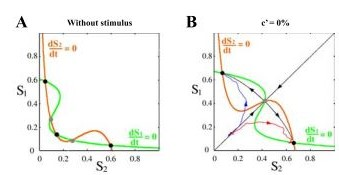
\includegraphics{fig/PhasePlaneAnalysisNoStimulus.jpg}
  \caption{Phase Plane Analysis of Reduced Model with unbiased stimulus}
  \label{fig:Phase Plane Analysis of Reduced Model}
\end{figure}
The model can also show delayed response version of the task. In this case, during the hold period, the choice is stored in either of the asymmetric stable nodes to be retrieved during decision making. A transient input post that can reset the model.

\begin{figure}
  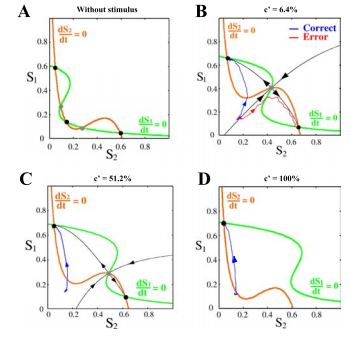
\includegraphics{fig/PhasePlaneAnalysisStimulus.jpg}
  \caption{Phase Plane Analysis of Reduced Model}
  \label{fig:Phase Plane Analysis of Reduced Model}
\end{figure}

This can be better visualised by a bifurcation diagram of selective population as function of stimulus strength $\mu_{0}$ as shown in Fig $3$. 

\begin{figure}
  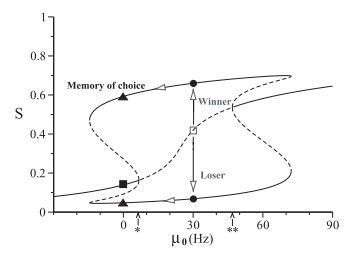
\includegraphics{fig/BifurcationDiagram.jpg}
  \caption{Bifurcation Diagram}
  \label{fig:Bifurcation Diagram}
\end{figure}

At the onset of the experiment, the state is at a stable steady state (filled square). With the introduction of a stimulus, the system translates to a unstable state (empty square). In this state, the system goes to either of the stable branches (either winning or losing choice). Further, on removal of the stimuli due to hysteresis of the state , the system continues to state in that state. Additionally at very high stimulus $\mu_{0} > 47$ Hz, one of the steady state (the losing choice) annhilates leaving only one steady state choice to the system.

$Fig 4$ shows the development of the phase plane in the presence of a biased stimuli with increasing $c \prime $ level. As can be seen with the increase in coherence, the  attractor basin of the biased choice becomes larger and finally above a particular critical coherence value , the attractor basin of the other choice annhilates (Fig $ 3.D$). Thus, above a particular $c \prime$ , the model would always select the correct choice. \\

The biased external stimuli which favours one of the choices can also be used to explain another experimental observation. As already mentioned, with an increase in $c \prime$, the probability of choosing the favoured choice increases. This happens as the spontaneous state of the system gets located deeper and deeper into the favoured attractor basin (Fig $3.C$). Thus noise and perturbations cannot dislocate the system into the stable manifold leading to extraction towards the saddle point or making an error choice. This location of spontaneous state deeper into the attractor basin of the favoured choice also explains decrease in decision time as the localtion of spontaneous stage makes it impervious to noise and leads to a quicker merging into attractor node. \\

Further, in case of trial error Fig $3.B$ (red line) in order for the model to make a error choice, it will first travel along the stable manifold and would later diverge away from it into the error attractor. This diverging away takes time due to the ruins of the attractor \cite{hubbard2012differential} leading to a comparatively longer decision time in case of error trails than correct trials.\\

As has been mentioned above in case of low $c \prime$ value, the system initiates in/near the stable manifold and first converges towards the saddle ; further any perturbation pushes it into the unstable manifold leading to one of the categorical choices. Thus, we would next analyse the impact of the saddle node and the ruins of attractor on the integration time in case of low coherence and weak input $\mu_{0}$. As the dynamics near the saddle is slow, the distance between S = $(S_{1}, S_{2})$ and $S_{saddle}$ can be linearised and expressed as :-\\

\indent $\Delta S = a_{1}v_{1}exp(-t/\tau_{stable}) + a_{2}v_{2}exp(-t/\tau_{unstable})$\\

Here, $v_{1}$ and $v_{2}$ are the eigenvectors of the saddle node (which is nothing but the stable and unstable manifolds). $\tau_{stable}$ and $\tau_{unstable}$ are the eigenvalues. $a_{1}$ and $a_{2}$ determined by the initial condition of the system, such that when the system initialises at the stable manifold the distance between the system and the saddle decreases in the order of $exp(-t/\tau_{stable})$ and if the system initialises in the unstable manifold , it distance between the system state and the saddle increases at a rate of $exp(-t/\tau_{unstable})$.


This linearization of the slow dynamics of the saddle area can successfully explain the longer decision time for weaker inputs $\mu_{0}$.

\begin{figure}
  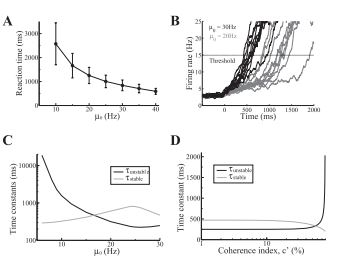
\includegraphics{fig/AnalysisSaddle.jpg}
  \caption{Slower dynamics due to Saddle}
  \label{fig:Phase Plane Analysis of Reduced Model}
\end{figure} 

 Looking in Fig $5. A$ and $5.C$ shows that with a decrease in $\mu_{0}$ the decision time increases , this increase can be paralleled with the increase in $\tau_{unstable}$ (which this model is able to show). However, this linearization tends to over emphasize the role of saddle on the system. First, it disregards the role of the stable manifold in the decision integration time , which cannot be ignored as the system's spontaneous stage lies on or near the stable manifold. Additionally, noise and increase in $c \prime$ pushes the system away from the saddle region, further diminishing their role on the integration time.

The model also tried to explain through phase plane is the role of NMDA synapses on the model. Inorder the elicit the role of NMDA synapses on the excitatory units, we have to reintroduce AMPA synapses into the model. This was achieved by using the 11 variable model definition of the reduced model phase. 







